\section{Material \& Methods}

\subsection{Data collection}
I collected data on body size of fossil testudinids from the Miocene until recent times. The body size data set includes 30 genera, comprising over 100 fossil species. The majority of the data was obtained from the primary literature (Table \ref{TabS1}). To find relevant publications, I relied mostly on the references listed in FosFarBase (CITE), PDBD (cite), and "Fossil Turtle Checklist (CITE).
Furthermore, the FosFarBase provided fossil occurences of testudinids all over the world, including their exact localities and age (Table \ref{TabS2}), which were used to get an overview over the availability of body size data. 
For extant taxa, I measured dry material (n = 67) from the collection of the Museum für Naturkunde zu Berlin (MFN). In addition, body size data from the literature was included (Table \ref{TabS3}).

\subsection{Body size estimation}
Body size is reported as straight carapace length (SCL). Where SCL was not available from the primary literature, it was estimated either from plastron length (PL) or appendicular elements (Table \ref{TabS1}). For carapace length estimations based on plastron length, the measurements from the MFN collection material was used to calculate the ratio between SCL and PL. Since the SC/PL ratio was similar for all species and genera, a single general ratio was calculated for all testudinids and hence used for the SCL estimations unless stated otherwise (Table \ref{TabS1}). For estimations based on femora and humeri, the ratio provided by Hutterer et al. (1998) and Franz et al. (2001), respectively, were used. A number of publications did not state measurements but instead provided scaled figures of the fossil remains, from which SCL, PL or humeri and femur lengths could be measured.

%TO DO: check Franz \& Quitmyer, 2005 again!! (CL regression)

\subsection{Analyses}
All subsequent analyses were performed with R (version 3.4.1), including the packages dplyr (cite) to prepare the data for the analysis (???) and ggplot2 (cite) to create figures. Sampling Accumulation Curves were created with the R package vegan (Cite) to see if sample size sufficed. This was repeated on genus level, since genera of fossil testudinids are relatively well resolved by now whereas determination on the species level is still somewhat obscure in many cases, as some species were based on scarce material. Since the data set relies on literature, occurrences increase with each added reference and reach a maximum, when no new species/genera are added.

% read Species Accumulation Curve papers + Catalinas paper!
% REWRITE

\subsubsection{Distribution and statistics}
Histograms and boxplots of the entire data set and several subgroups (fossil vs. modern, insular vs. continental...) were created to explore the distribution of body size. The Wilcoxon Rank Sum Test (unpaired data) was used to test for differences between two subgroups. To be able to compare different subgroups, a subsample (1000 repeats) of the respective larger subgroup was taken to compare equal sample sizes. 

%- only used samples > 23.000 mya?!

\subsubsection{Body size trends over time}
To investigate trends in body size over time, the R package paleoTS (cite) was used. Data were split into time bins according to the stratigraphic timescale/stages (Table \ref{tab:bins}, Fig. \ref{fig:bins}). Data older than 23 mya was excluded from the final analysis. To decrease influenec of sampling bias and because Sampling Accumulation Curves showed that the genus level was well sampled in contrast to species level, the mean SCL per genus was calculated before the timescale analysis. The paleoTS plots were created, wich display the mean trait over time and can be fitted to different evolutionary models: stasis, which ...., generalized random walk (GRW), which .... or unbiased random walk (URW), which..... . The Akaike Weight Criterion (AICc) indicates which model is best supported --> see Catalina's Paper and Hunt's papers


\begin{figure}[htbp]
	\centering
	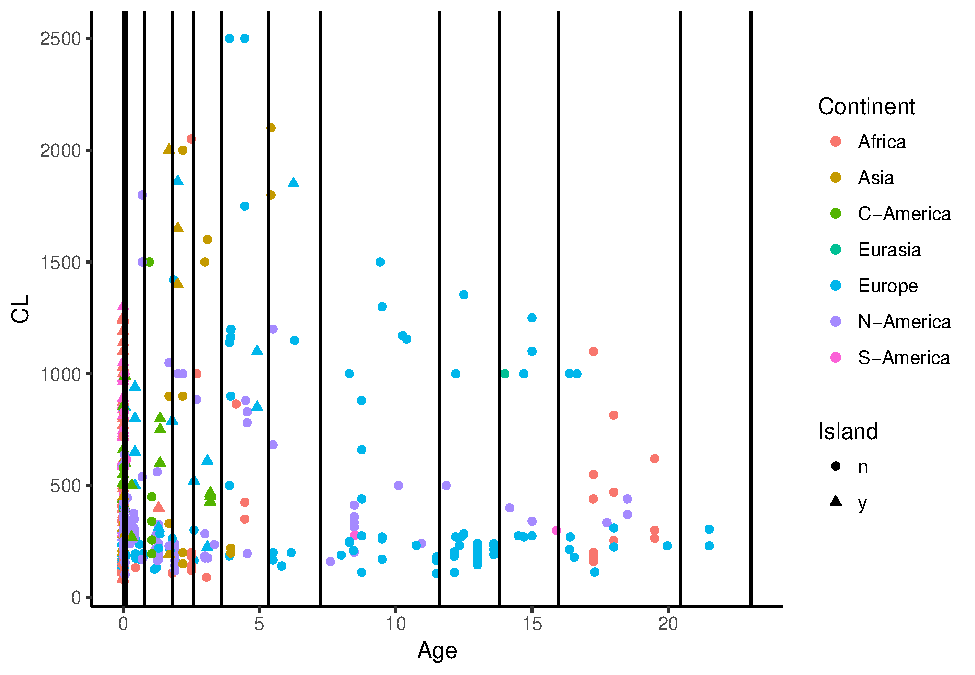
\includegraphics{MA_JJ_files/figure-latex/overview.pdf}
	\caption{Scatterplot of carapace length over time, indicating insular (triangle) and
		continental (circles) and colour indicating continents. Lines indicate time
		bins which correspons to stratigraphic stages.}
	\label{fig:bins}
\end{figure}
